\section{Definitions}
\subsection{IoT and IIoT}
\subsection{IoT-Platforms}
\section{State of the art}
\subsection{Industrial IoT Architectures and Patterns}
Due to the requirement that the solution be developed utilizing IoT technologies and is set within a production context, a review of Industrial IoT (IIoT) architectures and patterns was conducted. The Industrial Internet Reference Architecture (IIRA) \cite{IIRA} serves as a comprehensive framework, offering valuable insights into various architectural models and design patterns relevant to this domain. This reference architecture describes the following patterns: IoT Component Capability Pattern, Three-Tier Architecture Pattern, Gateway-Mediated Edge Connectivity and Management architecture pattern, Digital Twin Core as a Middleware Architecture Pattern, Layered Databus Architecture Pattern, System-of-Systems Orchestrator Architecture Pattern. Of these patterns only the first two are applicable within the scope of this work. Therefore the other ones will only be described on the surface.
\paragraph{Architecture Patterns}
IoT architecture patterns define the structure and operation of various IoT systems, detailing their implementation and highlighting their unique characteristics.
\subparagraph{IoT Component Capability Model Pattern}
A single component and its associated capabilities are described, with the possibility that a component may comprise multiple sub-components. Consequently, the entire system can also be regarded as a component. The specific meanings of the capabilities are illustrated in the accompanying figure.
\begin{figure}
	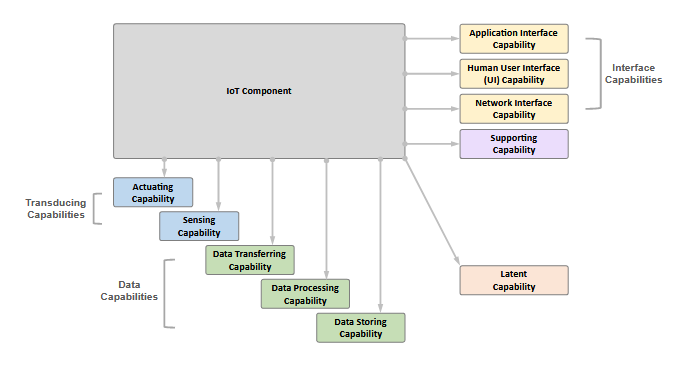
\includegraphics[width=\linewidth]{images/IIRA-model-component-pattern.png}
	\caption{Component Capability Pattern.}
	\label{fig:boat1}
\end{figure}
\subparagraph{Three-Tier Architecture Pattern}
The system is comprised of the Edge-, Platform- and Enterprise Tier as well as connecting networks. The edge tier holds the sensors and gateways to collect data. These are connected by the proximity network. There is possible for data preprocessing to already be happening there.
The platform tier is responsible for most of the data processing and storage via databases.
\subsection{Performance measurement in production environments}
\subsection{IoT-Plattforms}
\subsection{Databases}
\subsection{Dashboarding}